% Method schematic (prompts, rollouts, detectors, analyses), file fig0-method.pdf.
% Build from paper/ so that fontspec's Path=fonts/ resolves, as in aes.sty:
%   xelatex -output-directory=<build dir> figures/method-diagram.tex
% Natural width 16.6 cm, the A4 text width: include at width=\textwidth with no rescaling.
% Strokes are inset from the bounding box so that none is clipped at the page edge.
\RequirePackage{fix-cm}
\documentclass[tikz]{standalone}
\usepackage{fontspec}
% Copied from aes.sty, lines 46 to 49.
\setmainfont{OpenSans}[
 Path=fonts/,Extension=.ttf,
 UprightFont=*-Regular,BoldFont=*-Bold,
 ItalicFont=*-Italic,BoldItalicFont=*-BoldItalic]
\usepackage{amsmath}
% Maths at 8.5 pt with scripts at 7.5 pt, so the prime of d' stays above the 7 pt floor with a
% margin. The paper's maths is Computer Modern; so is the figure's.
\DeclareMathSizes{8.5}{8.5}{7.5}{7}
% The agreement scale sets kappa at 9.5 pt with a 7 pt subscript, the ratio of the paper's kappa_max.
\DeclareMathSizes{9.5}{9.5}{7}{7}
\DeclareMathSizes{8}{8}{7.5}{7}
\DeclareMathSizes{7.5}{7.5}{7}{7}
\usetikzlibrary{calc,arrows.meta,decorations.pathreplacing,patterns}
% Colours copied from aes.sty, lines 53 to 58.
\definecolor{aesink}{HTML}{090C27}
\definecolor{aespurple}{HTML}{6658E8}
\definecolor{bodyink}{HTML}{111318}
\definecolor{secondary}{HTML}{454754}
% Two greys for everything neutral; the purple family only for what a detector reads.
\colorlet{gline}{black!45}
\colorlet{glight}{black!15}
\colorlet{readfill}{aespurple!55}
\colorlet{readline}{aespurple!75!black}
\colorlet{givenfill}{aespurple!20}
\colorlet{givenline}{aespurple!80}   % about 3.5:1 on white

% Text sizes: 10.5 pt stage headings; 8 pt names and labels (bold only for detector names and
% the two analysis titles); 7.5 pt notes; 7 pt only inside the cue tags.
\newcommand{\head}{\fontsize{10.5}{12.6}\selectfont}
\newcommand{\eight}{\fontsize{8}{9.6}\selectfont}
\newcommand{\note}{\fontsize{7.5}{8.8}\selectfont}
\newcommand{\tagsize}{\fontsize{7}{8}\selectfont}
\newcommand{\mth}{\fontsize{8.5}{10}\selectfont}
\newcommand{\mthscale}{\fontsize{9.5}{11}\selectfont}
\hyphenpenalty=10000\exhyphenpenalty=10000

\begin{document}
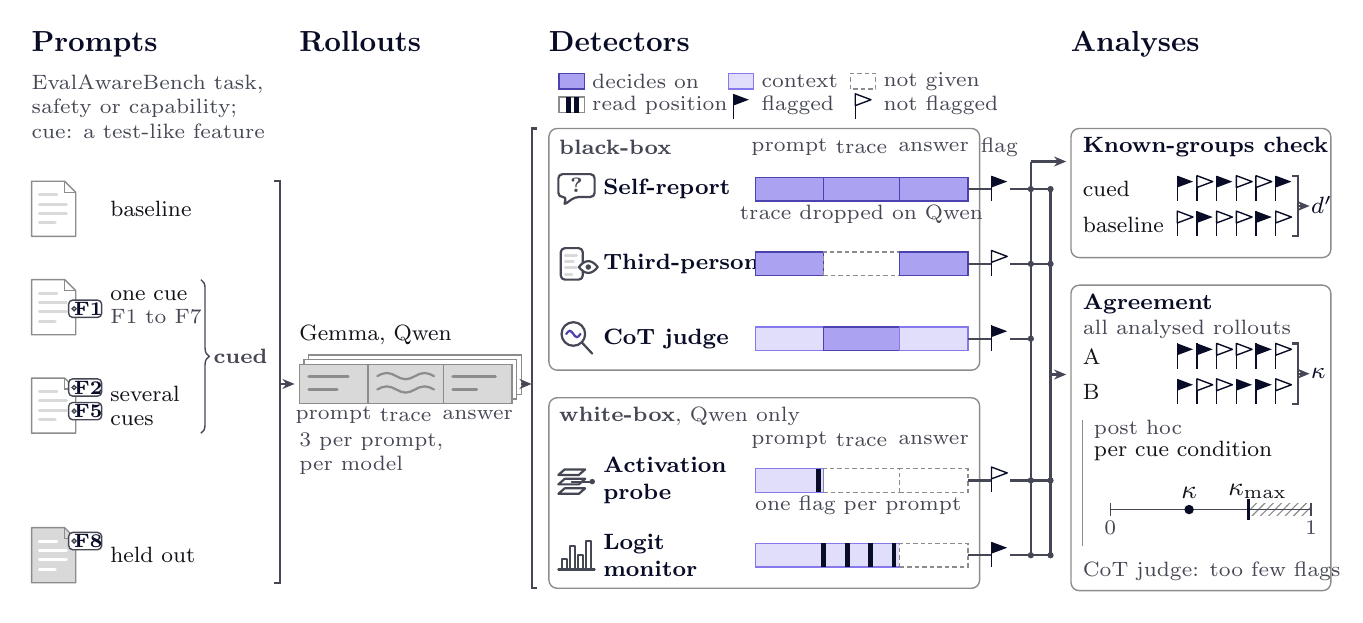
\begin{tikzpicture}[x=1cm,y=1cm,
  every node/.style={inner sep=0pt,outer sep=0pt,font=\eight,text=bodyink},
  stage/.style={font=\head\bfseries,text=aesink,anchor=north west},
  dname/.style={font=\eight\bfseries,text=aesink,anchor=west,align=left},
  note/.style={font=\note,text=secondary},
  grp/.style={font=\note\bfseries,text=secondary},
  % three strokes: 0.5 pt outlines, 0.8 pt connectors and glyphs, 1.1 pt lines of text
  ln/.style={line width=0.5pt},
  conn/.style={line width=0.8pt,color=secondary},
  arr/.style={conn,-{Stealth[length=4.4pt,width=3.6pt]}},
  glyph/.style={line width=0.8pt,draw=secondary,line join=round,line cap=round},
  txt/.style={line width=1.1pt,line cap=round},
  % two corner radii: 3 pt for enclosures, 1.5 pt for tags and glyphs
  panel/.style={ln,draw=gline,fill=white,rounded corners=3pt},
  % the three states of a rollout part, for one detector
  sdec/.style={ln,draw=readline,fill=readfill},
  sctx/.style={ln,draw=givenline,fill=givenfill},
  snot/.style={ln,draw=gline,fill=white,dash pattern=on 1.6pt off 1.1pt},
]
\useasboundingbox (0,0) rectangle (16.6,7.2);

% ================================================================ grid
% columns (cm)
\def\xA{0.05}      % prompts: page left edge
\def\xAl{1.05}     % prompts: labels
\def\xAbr{2.2}     % the brace that groups the cued prompts
\def\xAbus{3.2}    % the line that gathers every prompt
\def\xB{3.45}      % rollout strip
\def\xCbus{6.40}   % the line that hands the rollout to every detector
\def\xC{6.62}      % detector regions, left edge
\def\xG{6.97}      % detector glyph centres
\def\xN{7.31}      % detector names
\def\xS{9.24}      % miniature strips
\def\xCr{12.09}    % detector regions, right edge
\def\xFl{12.24}    % flags
\def\xKb{12.74}    % bus to the known-groups check (all five detectors)
\def\xAb{12.99}    % bus to agreement (all but the CoT judge)
\def\xD{13.25}     % analysis panels
\def\xDr{16.55}
\def\pad{0.15}     % one left inset for both analysis panels
\def\xF{14.6}      % first flag in both analysis panels
\def\fp{0.25}      % one flag pitch in both analysis panels
% rollout parts: one strip width (2.7 cm) for the rollout and its miniatures
\def\wP{0.87}\def\wT{0.96}\def\wA{0.87}
% rows (cm): one 0.95 pitch for the detectors
\def\yHead{7.15}
\def\yMid{2.675}   % the flow line: prompts, rollout and detectors share it
\def\yBBt{5.92}\def\yBBh{5.68}\def\yBBb{2.85}
\def\yWBt{2.5}\def\yWBh{2.27}\def\yWBp{1.96}\def\yWBb{0.08}
\def\yR{5.15}\def\yRR{4.2}\def\yRRR{3.25}\def\yRRRR{1.45}\def\yRRRRR{0.5}

% ================================================================ glyphs
% A flag, the output of a detector for one rollout. #3: flagged (filled) or not (hollow).
\newcommand{\flag}[3]{%
  \draw[ln,color=aesink] (#1,#2-0.15) -- (#1,#2+0.17);
  \ifnum#3=1
    \fill[aesink] (#1,#2+0.17) -- (#1+0.2,#2+0.095) -- (#1,#2+0.02) -- cycle;
  \else
    \draw[ln,draw=aesink,fill=white,line join=round] (#1,#2+0.17) -- (#1+0.2,#2+0.095) -- (#1,#2+0.02) -- cycle;
  \fi}
% A prompt: a page with a folded corner and lines of text. #1 fill, #2 text-line colour.
\newcommand{\page}[4]{% fill textcolour x y (lower left)
  \draw[ln,draw=gline,fill=#1,line join=round]
    (#3,#4) -- (#3+0.56,#4) -- (#3+0.56,#4+0.56) -- (#3+0.42,#4+0.7) -- (#3,#4+0.7) -- cycle;
  \draw[ln,draw=gline] (#3+0.42,#4+0.7) -- (#3+0.42,#4+0.56) -- (#3+0.56,#4+0.56);
  \foreach \l/\e in {0.53/0.32,0.41/0.44,0.29/0.44,0.17/0.3}{
    \draw[txt,color=#2] (#3+0.1,#4+\l) -- (#3+\e,#4+\l);}}
% A cue: a tag hung on the page's right edge.
\newcommand{\cue}[3]{% x y (left middle) label
  \draw[ln,draw=secondary,fill=white,rounded corners=1.5pt]
    (#1,#2-0.11) rectangle (#1+0.42,#2+0.11);
  \draw[line width=0.5pt,draw=secondary] (#1+0.07,#2) circle (0.025);
  \node[font=\tagsize\bfseries,text=aesink] at (#1+0.25,#2) {#3};}
% A rollout: prompt, trace and answer as one strip. #1 x, #2 y (centre), #3 height,
% #4/#5/#6 the style of each part.
\newcommand{\strip}[6]{%
  \draw[#4] (#1,#2-#3/2) rectangle (#1+\wP,#2+#3/2);
  \draw[#5] (#1+\wP,#2-#3/2) rectangle (#1+\wP+\wT,#2+#3/2);
  \draw[#6] (#1+\wP+\wT,#2-#3/2) rectangle (#1+\wP+\wT+\wA,#2+#3/2);}
\newcommand{\partlabels}[2]{% x y: the names of the three parts, centred on them
  \node[note] at (#1+0.5*\wP,#2) {prompt};
  \node[note] at (#1+\wP+0.5*\wT,#2) {trace};
  \node[note] at (#1+\wP+\wT+0.5*\wA,#2) {answer};}
% Detector glyphs: one box (about 0.46 x 0.42 cm), one stroke, one colour, line art only.
\newcommand{\gselfreport}[2]{% a speech bubble with a question
  \draw[glyph,fill=white,rounded corners=1.5pt]
    (#1-0.23,#2-0.1) -- (#1-0.12,#2-0.1) -- (#1-0.17,#2-0.21) -- (#1-0.02,#2-0.1)
    -- (#1+0.23,#2-0.1) -- (#1+0.23,#2+0.19) -- (#1-0.23,#2+0.19) -- cycle;
  \node[font=\note\bfseries,text=secondary] at (#1,#2+0.045) {?};}
\newcommand{\gthirdperson}[2]{% a transcript sheet, read by an eye from outside
  \draw[glyph,fill=white,rounded corners=1.5pt] (#1-0.2,#2-0.2) rectangle (#1+0.08,#2+0.2);
  \foreach \l/\e in {0.11/0.0,0.03/-0.04,-0.05/0.0,-0.13/-0.06}{
    \draw[txt,color=glight] (#1-0.14,#2+\l) -- (#1+\e,#2+\l);}
  \draw[glyph,fill=white] (#1+0.03,#2-0.04) .. controls (#1+0.11,#2+0.06) and (#1+0.19,#2+0.06) .. (#1+0.27,#2-0.04)
    .. controls (#1+0.19,#2-0.14) and (#1+0.11,#2-0.14) .. cycle;
  \fill[secondary] (#1+0.15,#2-0.04) circle (0.035);}
\newcommand{\gcotjudge}[2]{% a magnifier over a line of reasoning
  \draw[glyph] (#1+0.07,#2-0.05) -- (#1+0.2,#2-0.19);
  \draw[glyph,fill=white] (#1-0.04,#2+0.06) circle (0.15);
  \draw[line width=0.8pt,color=readline,line cap=round]
    (#1-0.13,#2+0.06) sin (#1-0.085,#2+0.1) cos (#1-0.04,#2+0.06) sin (#1+0.005,#2+0.02) cos (#1+0.05,#2+0.06);}
\newcommand{\gprobe}[2]{% stacked layers, one pierced by a probe
  \foreach \k in {0,1,2}{
    \draw[glyph,fill=white] (#1-0.23,#2-0.17+0.12*\k) -- (#1+0.03,#2-0.17+0.12*\k)
      -- (#1+0.11,#2-0.1+0.12*\k) -- (#1-0.15,#2-0.1+0.12*\k) -- cycle;}
  \draw[glyph] (#1-0.06,#2-0.015) -- (#1+0.2,#2-0.015);
  \fill[secondary] (#1+0.2,#2-0.015) circle (0.035);}
\newcommand{\glogit}[2]{% token probabilities as small outlined bars on a baseline
  \draw[glyph] (#1-0.23,#2-0.18) -- (#1+0.23,#2-0.18);
  \foreach \i/\h in {-0.15/0.13,-0.05/0.3,0.05/0.18,0.15/0.36}{
    \draw[glyph,fill=white] (#1+\i-0.03,#2-0.18) rectangle (#1+\i+0.03,#2-0.18+\h);}}
% a junction on a bus
\newcommand{\jdot}[2]{\fill[secondary] (#1,#2) circle (0.04);}
% a gather bracket: a vertical line with ticks pointing at what it gathers. #1 x, #2 top,
% #3 bottom, #4 tick direction (+1 right, -1 left)
\newcommand{\gatherline}[4]{%
  \draw[conn] (#1+#4*0.07,#2) -- (#1,#2) -- (#1,#3) -- (#1+#4*0.07,#3);}

% ================================================================ 1. Prompts
\node[stage] at (\xA,\yHead) {Prompts};
\node[note,anchor=north west,align=left] at (\xA,6.6)
  {EvalAwareBench task,\\safety or capability;\\cue: a test-like feature};
% baseline: no cue
\page{white}{glight}{\xA}{4.55}
\node[anchor=west] at (\xAl,4.9) {baseline};
% one cue
\page{white}{glight}{\xA}{3.3}
\cue{\xA+0.47}{3.63}{F1}
\node[anchor=west,align=left] at (\xAl,3.65) {one cue\\[-1pt]{\note\color{secondary}F1 to F7}};
% several cues
\page{white}{glight}{\xA}{2.05}
\cue{\xA+0.47}{2.63}{F2}
\cue{\xA+0.47}{2.33}{F5}
\node[anchor=west,align=left] at (\xAl,2.4) {several\\[-1pt]cues};
% cued = one cue or several
\draw[decorate,decoration={brace,amplitude=3pt},ln,color=secondary]
  (\xAbr,4.0) -- (\xAbr,2.05) coordinate[midway] (cued);
\node[grp,anchor=west] at ($(cued)+(0.16,0)$) {cued};
% F8: rolled out but held out of the analyses; a grey page, not a dashed one
\page{glight}{white}{\xA}{0.15}
\cue{\xA+0.47}{0.68}{F8}
\node[anchor=west] at (\xAl,0.5) {held out};
% every prompt, F8 included, is rolled out
\gatherline{\xAbus}{5.25}{0.15}{-1}
\draw[arr] (\xAbus,\yMid) -- (\xB-0.06,\yMid);

% ================================================================ 2. Rollouts
\node[stage] at (\xB,\yHead) {Rollouts};
% design/reps = 3: two offset copies behind the front strip
\foreach \s in {0.12,0.06}{
  \draw[ln,draw=gline,fill=white] (\xB+\s,\yMid-0.25+\s) rectangle (\xB+\wP+\wT+\wA+\s,\yMid+0.25+\s);}
\strip{\xB}{\yMid}{0.5}{ln,draw=gline,fill=glight}{ln,draw=gline,fill=glight}{ln,draw=gline,fill=glight}
% lines of text inside each part; the trace drawn as loose reasoning
\foreach \l/\e in {0.1/0.62,-0.07/0.48}{
  \draw[txt,color=gline] (\xB+0.12,\yMid+\l) -- (\xB+\e,\yMid+\l);}
\foreach \l in {0.1,-0.07}{
  \draw[line width=0.8pt,color=gline,line cap=round]
    (\xB+\wP+0.12,\yMid+\l) sin (\xB+\wP+0.24,\yMid+\l+0.04) cos (\xB+\wP+0.36,\yMid+\l)
    sin (\xB+\wP+0.48,\yMid+\l-0.04) cos (\xB+\wP+0.6,\yMid+\l) sin (\xB+\wP+0.72,\yMid+\l+0.04)
    cos (\xB+\wP+0.84,\yMid+\l);}
\foreach \l/\e in {0.1/0.66,-0.07/0.42}{
  \draw[txt,color=gline] (\xB+\wP+\wT+0.12,\yMid+\l) -- (\xB+\wP+\wT+\e,\yMid+\l);}
\node[anchor=south west] at (\xB,\yMid+0.5) {Gemma, Qwen};
\partlabels{\xB}{\yMid-0.4}
% design/reps = 3
\node[note,anchor=north west,align=left] at (\xB,\yMid-0.62) {3 per prompt,\\per model};
\draw[arr] (\xB+\wP+\wT+\wA+0.12,\yMid) -- (\xCbus,\yMid);

% ================================================================ 3. Detectors
\node[stage] at (\xC,\yHead) {Detectors};
% key, read before the rows: three cell states, the read positions, the two flag states
\def\kA{\xC+0.13}\def\kB{\xC+2.28}\def\kC{\xC+3.83}
\def\yKa{6.52}\def\yKb{6.22}
\newcommand{\keycell}[3]{% x style label
  \draw[#2] (#1,\yKa-0.1) rectangle (#1+0.32,\yKa+0.1);
  \node[note,anchor=west] at (#1+0.42,\yKa) {#3};}
\keycell{\kA}{sdec}{decides on}
\keycell{\kB}{sctx}{context}
\keycell{\kC}{snot}{not given}
\draw[ln,draw=gline,fill=white] (\kA,\yKb-0.1) rectangle (\kA+0.32,\yKb+0.1);
\fill[aesink] (\kA+0.09,\yKb-0.1) rectangle (\kA+0.15,\yKb+0.1);
\fill[aesink] (\kA+0.19,\yKb-0.1) rectangle (\kA+0.25,\yKb+0.1);
\node[note,anchor=west] at (\kA+0.42,\yKb) {read position};
\flag{\kB+0.06}{\yKb-0.03}{1}
\node[note,anchor=west] at (\kB+0.42,\yKb) {flagged};
\flag{\kC+0.06}{\yKb-0.03}{0}
\node[note,anchor=west] at (\kC+0.42,\yKb) {not flagged};

% the rollout reaches every detector
\gatherline{\xCbus}{\yBBt}{\yWBb}{1}

% two regions at one level, neutral: black-box and white-box
\draw[panel] (\xC,\yBBb) rectangle (\xCr,\yBBt);
\draw[panel] (\xC,\yWBb) rectangle (\xCr,\yWBt);
\node[grp,anchor=west] at (\xC+0.13,\yBBh) {black-box};
\node[grp,anchor=west] at (\xC+0.13,\yWBh) {white-box\textmd{, Qwen only}};
\partlabels{\xS}{\yBBh}
\partlabels{\xS}{\yWBp}
\node[note] at (\xFl+0.1,\yBBh) {flag};

% one detector: glyph, name, the rollout in miniature, a line to its flag
\newcommand{\detector}[7]{% y glyph name s1 s2 s3 flagged
  #2{\xG}{#1}
  \node[dname] at (\xN,#1) {#3};
  \strip{\xS}{#1}{0.3}{#4}{#5}{#6}
  \draw[conn] (\xS+\wP+\wT+\wA,#1) -- (\xFl,#1);
  \flag{\xFl}{#1}{#7}}

\detector{\yR}{\gselfreport}{Self-report}{sdec}{sdec}{sdec}{1}
% Qwen's chat template (6a9e13bd) drops the reasoning of earlier assistant turns, so on Qwen
% self-report sees the task and the answer only. Gemma's published template keeps the trace as
% text, but Gemma ran on API providers whose template copy we cannot see; only Qwen is stated.
\node[note,anchor=north] at (\xS+\wP+0.5*\wT,\yR-0.2) {trace dropped on Qwen};
\detector{\yRR}{\gthirdperson}{Third-person}{sdec}{snot}{sdec}{0}
\detector{\yRRR}{\gcotjudge}{CoT judge}{sctx}{sdec}{sctx}{1}

\detector{\yRRRR}{\gprobe}{Activation\\probe}{sctx}{snot}{snot}{0}
% read position: the last prompt token
\fill[aesink] (\xS+\wP-0.1,\yRRRR-0.15) rectangle (\xS+\wP-0.04,\yRRRR+0.15);
\node[note,anchor=north west] at (\xS,\yRRRR-0.2) {one flag per prompt};

\detector{\yRRRRR}{\glogit}{Logit\\monitor}{sctx}{sctx}{snot}{1}
% read positions: the start of the trace, then points spread evenly along it
% (design/logitpositions caps them; drawn as four, a symbol for several)
\foreach \f in {0,0.31,0.62,0.93}{
  \fill[aesink] (\xS+\wP+\f*\wT-0.03,\yRRRRR-0.15) rectangle (\xS+\wP+\f*\wT+0.03,\yRRRRR+0.15);}

% flags to the analyses: every flag reaches the known-groups bus; all but the CoT judge's
% continue to the agreement bus
\foreach \y in {\yR,\yRR,\yRRRR,\yRRRRR}{
  \draw[conn] (\xFl+0.24,\y) -- (\xAb,\y);
  \jdot{\xKb}{\y}\jdot{\xAb}{\y}}
\draw[conn] (\xFl+0.24,\yRRR) -- (\xKb,\yRRR);
\jdot{\xKb}{\yRRR}
\draw[conn] (\xKb,\yRRRRR) -- (\xKb,5.5);
\draw[arr] (\xKb,5.5) -- (\xD-0.06,5.5);
\draw[conn] (\xAb,\yR) -- (\xAb,\yRRRRR);
\draw[arr] (\xAb,2.795) -- (\xD-0.06,2.795);

% ================================================================ 4. Analyses
\node[stage] at (\xD,\yHead) {Analyses};
% ---- known-groups check: flags on cued rollouts against flags on baseline rollouts
\def\yKGt{\yBBt}\def\yKGbot{4.28}
\def\yKGa{5.15}\def\yKGb{4.7}
\draw[panel] (\xD,\yKGbot) rectangle (\xDr,\yKGt);
\node[dname] at (\xD+\pad,\yBBh) {Known-groups check};
\node[anchor=west] at (\xD+\pad,\yKGa) {cued};
\node[anchor=west] at (\xD+\pad,\yKGb) {baseline};
% mixed on purpose: the schematic shows the comparison, not its result
\foreach \i/\r in {0/1,1/0,2/1,3/0,4/0,5/1}{\flag{\xF+\fp*\i}{\yKGa}{\r}}
\foreach \i/\r in {0/0,1/1,2/0,3/0,4/1,5/0}{\flag{\xF+\fp*\i}{\yKGb}{\r}}
\def\xGa{16.13}
\gatherline{\xGa}{\yKGa+0.17}{\yKGb-0.15}{-1}
\draw[arr] (\xGa,{(\yKGa+\yKGb)/2+0.01}) -- (\xGa+0.15,{(\yKGa+\yKGb)/2+0.01});
\node[font=\mth,text=aesink,anchor=west] at (\xGa+0.17,{(\yKGa+\yKGb)/2+0.02}) {$d'$};

% ---- agreement: two detectors' flags on the same rollouts
\def\yAGt{3.93}\def\yAGb{0.05}
\def\yAa{3.02}\def\yAb{2.57}
\draw[panel] (\xD,\yAGb) rectangle (\xDr,\yAGt);
\node[dname] at (\xD+\pad,3.69) {Agreement};
% the planned analysis, at full weight
\node[note,anchor=west] at (\xD+\pad,3.37) {all analysed rollouts};
\node[anchor=west] at (\xD+\pad,\yAa) {A};
\node[anchor=west] at (\xD+\pad,\yAb) {B};
% mixed on purpose: the schematic shows the comparison, not its result
\foreach \i/\r in {0/1,1/1,2/0,3/0,4/1,5/0}{\flag{\xF+\fp*\i}{\yAa}{\r}}
\foreach \i/\r in {0/1,1/0,2/0,3/1,4/1,5/0}{\flag{\xF+\fp*\i}{\yAb}{\r}}
\gatherline{\xGa}{\yAa+0.17}{\yAb-0.15}{-1}
\draw[arr] (\xGa,{(\yAa+\yAb)/2+0.01}) -- (\xGa+0.15,{(\yAa+\yAb)/2+0.01});
\node[font=\mth,text=aesink,anchor=west] at (\xGa+0.17,{(\yAa+\yAb)/2+0.02}) {$\kappa$};
% the post hoc analysis, lighter: a plain rule (no ticks, so not a gather) and a small label
\draw[ln,color=gline] (\xD+\pad,2.22) -- (\xD+\pad,0.62);
\node[note,anchor=west] at (\xD+\pad+0.14,2.1) {post hoc};
\node[anchor=west] at (\xD+\pad+0.14,1.82) {per cue condition};
% Cohen's kappa against the maximum kappa_max that the two positive rates allow; no numbers
\def\yS{1.08}\def\sL{13.75}\def\sR{16.3}
\def\xKmax{15.5}\def\xKap{14.75}
\fill[pattern=north east lines,pattern color=gline] (\xKmax,\yS-0.08) rectangle (\sR,\yS+0.08);
\draw[ln,color=secondary] (\sL,\yS) -- (\sR,\yS);
\draw[ln,color=secondary] (\sL,\yS-0.08) -- (\sL,\yS+0.08);
\draw[ln,color=secondary] (\sR,\yS-0.08) -- (\sR,\yS+0.08);
\draw[line width=1.1pt,color=aesink] (\xKmax,\yS-0.13) -- (\xKmax,\yS+0.13);
\node[anchor=south,font=\mthscale] at (\xKmax+0.12,\yS+0.14) {$\kappa_{\max}$};
\fill[aesink] (\xKap,\yS) circle (0.06);
\node[anchor=south,font=\mthscale] at (\xKap,\yS+0.14) {$\kappa$};
\node[note,anchor=north] at (\sL,\yS-0.15) {0};
\node[note,anchor=north] at (\sR,\yS-0.15) {1};
\node[note,anchor=west] at (\xD+\pad,0.3) {CoT judge: too few flags};
\end{tikzpicture}
\end{document}
